This chapter summarizes previous efforts in numerical simulations of prismatic HTGRs.
The simulation of prismatic HTGRs require the coupled modeling of the neutronics and thermal-fluid phenomena.
This chapter comprehends the following sections: Section \ref{sec:litreview-neut} addresses diffusion methods for solving the neutronics, Section \ref{sec:litrev-thermalf} focuses on the thermal-fluids, and Section \ref{sec:litreview-multi} studies the coupled simulations.

\section{Prismatic HTGR Diffusion Solvers}
\label{sec:litreview-neut}

Currently, several software programs solve the neutronics of prismatic \glspl{HTGR}.
Most of these programs rely on one of the following methods: stochastic transport (Monte Carlo), deterministic transport, or deterministic diffusion.
This section focuses on the last class.
% If time permits work on a brief description of the Monte Carlo and deterministic transport maybe.
% Why? Deterministic diffusion solvers have lower computational requirements than other methods reference ??
% The utilization of the Monte Carlo codes is unattractive because of the tremendous problem size and the need for a large number of neutron histories \cite{lee_status_2006}.
% It is one of the simplest means to solve neutron transport problems \cite{leppanen_development_2007}.
% Here I say the following
% Deterministic diffusion methods are computationally cheaper than the other methods.
% This characteristic makes it a good candidate for coupled calculations.

The history of deterministic diffusion solvers began in the late 1950s with the \gls{FDM} application to the analysis of \glspl{LWR}.
In \gls{FDM}, mesh spacings are usually of the order of the diffusion length.
While solving large multi-dimensional problems, this feature causes the mesh points to reach intractable numbers \cite{lewis_finite_1986}.
The computational expense of these calculations motivated the generation of more computationally efficient techniques \cite{lawrence_progress_1986}.
Although substantial overlaps exist, the most common techniques fall into two broad categories: nodal methods and \gls{FEM}.

% NODAL
FLARE \cite{delp_flare_1964} is a three-dimensional \gls{BWR} simulator, and it is representative of the first generation of nodal methods.
This approach used adjusted parameters to match actual operating data or the results of more accurate calculations.
Most of these methods were implementations of the so-called "1.5 group theory" \cite{gupta_nodal_1981}.
The second generation of nodal methods derived spatial coupling relationships by applying the \gls{TIP}.
This procedure obtains equivalent one-dimensional equations by integrating the multi-dimensional diffusion equation over directions transverse to each coordinate axis \cite{lawrence_progress_1986}.
This approach proved to be highly efficient and accurate in Cartesian geometries.

In 1981, a formulation based on the \gls{NEM} first demonstrated the feasibility of nodal methods in hexagonal geometries \cite{duracz_nodal_1981}.
However, this method would introduce non-physical singular terms that required the utilization of discontinuous polynomials.
This drawback motivated the development of more effective formulations.
HEXNOD, introduced in 1988 by Wagner \cite{wagner_three-dimensional_1989}, is an example of such formulations.
This algorithm uses the \gls{TIP} and, in contrast to the \gls{NEM}, solves the resulting differential equation analytically.
Wagner's article demonstrated the method's good accuracy by comparing to \gls{FDM} and Monte Carlo calculations for a few benchmark problems.

HEXPEDITE \cite{fitzpatrick_hexpedite_1992} introduced a new method that is another example of more effective formulations.
HEXPEDITE uses the \gls{TIP} formulation to derive a pseudo-one-dimensional equation.
The resulting differential equation is solved analytically.
The difference from HEXNOD is that HEXPEDITE uses a simpler and more efficient coupling scheme.
Different works \cite{fitzpatrick_hexpedite_1992}\cite{fitzpatrick_developments_1995} on the HEXPEDITE methodology tested the approach against the \gls{NEM} and the \gls{FDM}.
These studies established HEXPEDITE’s superiority in terms of accuracy and runtime.
HEXPEDITE's use prevailed in the analysis of \glspl{HTGR} until recently.
In 2010, \gls{INL} conducted a study \cite{ortensi_deterministic_2010-1} in which they compared HEXPEDITE's results against several diffusion solvers, as well as the Monte Carlo solvers MCNP5 \cite{rsicc_computer_code_collection_mcnp5_2003} and Serpent \cite{leppanen_serpent_2015}.

DIF3D \cite{lawrence_dif3d_1983} and PARCS \cite{downar_parcs_2004} are other examples of prevalent nodal diffusion tools.
DIF3D has several solution options such as the diffusion \gls{FDM}, diffusion \gls{NEM} based on \gls{TIP}, and the VARIANT nodal transport method.
% VARIANT: variational nodal \cite{palmiotti_variant_1995}
PARCS has several solution options as well, such as a diffusion \gls{FDM}, diffusion \gls{NEM} based on \gls{TIP}, P$_{N}$ transport methods, and the multigroup transport simplified P$_3$ with \gls{FDM} and \gls{NEM} discretizations.

% from ortensi_deterministic_2010-1 and wang_modified_2018
Nodal methods solve relatively coarse meshes for approximate solutions.
This characteristic makes the process efficient.
On the other hand, the method does not provide detailed point-wise accurate solutions \cite{kang_finite_1973}.
Additionally, the derivation of nodal methods happens in a specific coordinate system for a particular node shape.
The application to complex problems is not flexible as different geometries require customized configurations.
This lack of flexibility limits the applications of nodal methods to regular geometries only.

% FEM
Moltres is a diffusion FEM application.
The FEM is a well-established method in applied mathematics and engineering.
FEM is a numerical technique for finding approximate solutions to partial differential equations by deriving their weak or variational form.
Most applications make \gls{FEM} preferable due to its flexibility in the treatment of curved or irregular geometries.
Also, the use of high order elements attains higher rates of convergence \cite{cavdar_finite_2004}.
The first engineering application of \gls{FEM} was in the field of structural engineering dating back to 1956.
In successive years, \gls{FEM} became the most extensively used technique in almost every branch of engineering.
\glspl{FEM} have several advantages over the nodal methods.
It provides flexibility in the geometry definition, a firm mathematical basis, ease in extension to the multi-group application, and detailed point-wise accurate solutions \cite{lee_development_2008}.

In 1973, Kang et al. \cite{kang_finite_1973} described the first application of \gls{FEM} to neutron diffusion theory.
The fundamental motivation for this development was the impractical application of the \gls{FDM} to three-dimensional problems.
In this early work, the author compared different \gls{FEM} approaches to the \gls{FDM} in one-dimensional and two-dimensional problems.
The studies showed a higher order of convergence achieved by the \gls{FEM}.
Throughout the last four decades, many software programs utilized the \gls{FEM} to solve the diffusion equation.
Some of the most recent software for diffusion simulations are CRONOS2 \cite{lautard_cronos_1990}, \gls{CAPP} \cite{lee_development_2011}, and Rattlesnake \cite{wang_rattlesnake_2019}.
The list of \gls{FEM} diffusion solvers is more extensive, but this thesis focuses on the best-documented software in the open literature.

% CRONOS
\gls{CEA} developed CRONOS2 \cite{lautard_cronos_1990} as part of the SAPHYR system.
CRONOS2 conducts steady-state and transient multi-group calculations, based on the diffusion equation or the transport equation using the S$_N$ method and a \gls{FDM} or a \gls{FEM} discretization.
In 2008, Damian et al. \cite{damian_vhtr_2008} presented the code suite NEPTHIS\cite{cavalier_presentation_2005}/CAST3M\cite{studer_cast3marcturus_2007}, software that relied on CRONOS2.
Section \ref{sec:litreview-multi} describes further the coupling scheme.

% CAPP
In 2008, the \gls{KAERI} published an article \cite{lee_development_2008} that presented CAPP.
Its purposes are to conduct steady-state core physics analysis, core depletion analysis, and core transient analysis.
The article validated the software with two benchmark problems: the IAEA PWR benchmark problem, and Phase I Exercise 1 of the OECD/NEA PBMR-400 Benchmark \cite{reitsma_oecd-neansc_2008}.
In 2011, Lee et al. published an article \cite{lee_development_2011} that extended the functionalities of CAPP to prismatic HTGRs.
To validate CAPP, they had to integrate a simplified thermal-fluids tool to the software.
Section \ref{sec:litreview-multi} describes the thermal-fluids tool and the coupling scheme.

% Proghorn and Rattlesnake
RattleSnake \cite{wang_rattlesnake_2019} is the MOOSE \cite{gaston_moose_2009} based application for simulating the transport equation.
\gls{INL} had initially developed Pronghorn \cite{novak_pronghorn_2018} to model \glspl{PBMR} \cite{strydom_inl_2013}.
The MOOSE neutronics kernel library Yak incorporated the neutron diffusion models initially in Pronghorn.
Currently, RattleSnake is the primary tool for solving the linearized Boltzmann neutron transport equation within MOOSE and relies heavily on Yak.
Various solvers are available under RattleSnake, including low-order multigroup diffusion, spherical harmonics transport, and discrete ordinates transport, all solved with the \gls{FEM}.
% Both RattleSnake and Pronghorn yielded the same exact results when using the continuous \gls{FEM} multigroup diffusion option in RattleSnake.

% strydom_inl_2013
In 2013, \gls{INL} conducted the OECD/NEA MHTGR-350 Benchmark \cite{oecd_nea_benchmark_2017}\cite{strydom_inl_2013} without further simplifications.
The \gls{INL} team solved Phase I Exercise 1 using INSTANT-P1 \cite{wang_krylov_2011}, Pronghorn, and RattleSnake.
INSTANT-P1 is a transport solver that relies on the spherical harmonics discretization of angles.
The results for Pronghorn and RattleSnake were identical, and all presented results exhibited good agreement with the benchmark results.

\subsection{Energy group structure analysis}
\label{sec:energy-struct}

% Number of energy groups impact over the calculations
In the context of this thesis, Moltres uses homogenized group constants previously generated by neutron transport solvers.
The choice of the energy group structure for the group constant homogenization affects the accuracy of the diffusion calculation.
The longer neutron mean free path in \glspl{HTGR} compared to \gls{LWR} increases the spectral interactions between elements.
For this reason, HTGR analyses require more energy groups than conventional \gls{LWR} analyses.
This section summarizes previous studies on the impact of the energy group structure over the diffusion calculations.

\gls{ANL} directed a study \cite{lee_status_2006} to compare the accuracy of nodal diffusion calculations employing different energy group structures.
The group constant homogenization used the DRAGON neutron transport solver and the diffusion calculations utilized the application DIF3D.
For the study, the ANL team implemented a one-dimensional fuel-reflector model in which they compared the solution accuracy using 4, 7, 8, 14, and 23 energy groups.
They also used alternative energy group structures for the same number of groups.
For simplicity, the authors used the homogenized fuel compact model and generated all the group constant at 300 K.
One of their conclusions was that the number of energy groups should be more than 4, and more than 6 would be sufficient for uranium fueled HTGRs.
Another finding was that the accuracy of the diffusion calculation is sensitive to the energy group boundaries.
% Mention something about the metrics of the study? To asses the accuracy, they compared the multiplication factor.

% \begin{figure}[htbp!]
% 	\centering
% 	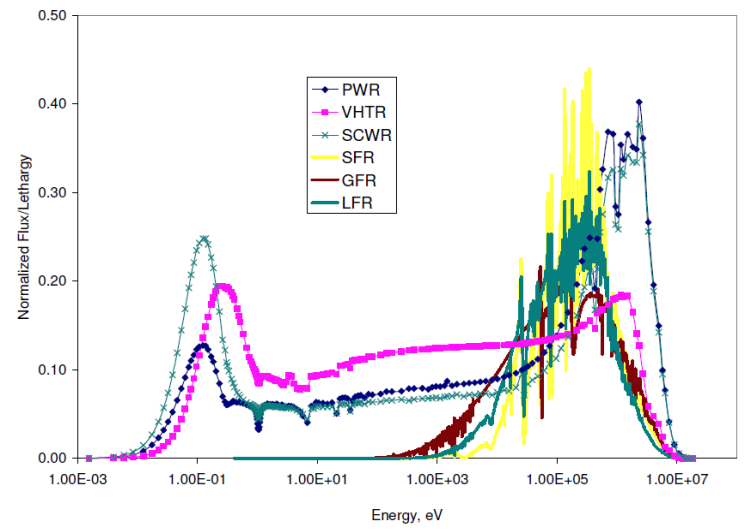
\includegraphics[width=0.40\linewidth]{figures/spectrum}
% 	\caption{Comparison of neutron energy spectra of different reactor designs. PWR=Pressurized Water Reactor, VHTR=Very High-Temperature Gas-Cooled Reactor, SCWR=Supercritical Water Reactor, SFR=Sodium Fast Reactor, GFR=Gas Fast Reactor, LFR=Lead Fast Reactor. Image reproduced from \cite{taiwo_summary_2005}.}
% 	\label{fig:spectrum}
% \end{figure}

% han_sensitivity_2008
Han's MS thesis \cite{han_sensitivity_2008} focused on selecting energy groups for the reactor analysis of the \gls{PBMR}.
The author used COMBINE6 \cite{grimesey_combinepc-portable_1994} for group constant generation and the Penn State nodal diffusion tool NEM \cite{bandini_three-dimensional_1990} for the reactor analysis.
The author compared the results against MCNP5 reference results.
To simplify the setup, the model used uniformly distributed isotopes in the fuel.
The study performed the calculations at 300 and 1000 K.
To arrive at an optimal group structure, the author compared many combinations of group structures using a trial and error strategy.
One conclusion of this work agrees with the previous bibliography \cite{gulf_oil_company_nuclear_1973} \cite{duderstadt_nuclear_1976} in that the energy spectrum is critical to yield an accurate description of a nuclear reactor using a few groups.

ANL's study helps set up proper nodal diffusion calculations for an \gls{HTGR}.
ANL's team conducted the study at 300 K --- not in the operational range of any \glspl{HTGR}.
On the contrary, Han's thesis included an analysis at 1000 K, and his results showed that the temperature changes have a non-negligible impact.
Additionally, ANL's study used the simplified model of the homogenized fuel compact.
Han highlighted that homogenized fuel models of the \gls{PBMR} underestimate criticality calculations.
In 2015, \gls{INL} presented their results \cite{strydom_results_2015} for an \gls{IAEA} coordinated research project \cite{tyobeka_htgr_2011} and showed that the homogenization of the compact material notably underestimates the multiplication factor.
On the other hand, the open literature has not widely investigated the impact of such simplification over the homogenized group constants.

\subsection{Summary of Prismatic HTGR Diffusion Solvers}

Section \ref{sec:litreview-neut} introduced several deterministic diffusion classes, including FDM, nodal methods, and FEM.
The fundamental motivation for the development of nodal methods and FEM was the impractical application of the \gls{FDM} to three-dimensional problems.
Section \ref{sec:litreview-neut} also discussed on the main characteristics of these methods, directing the reader's attention to the advantages of the FEM.
Although nodal methods are efficient, most applications make FEMs preferable due to its flexibility in the treatment of irregular geometries.
Additionally, FEMs have a firm mathematical basis, and its formulation eases the extension to multi-group applications.
Moltres relies on the FEM counting with all the advantages of the method.

Section \ref{sec:litreview-neut} summarized previous efforts in deterministic diffusion solvers of prismatic HTGRs.
This thesis draws two main conclusions from those earlier efforts.
The first conclusion is that several authors validated their solvers by comparison to other tools.
In the context of this thesis, Chapter \ref{ch:neutronics} describes two exercises: first, a comparison between Moltres and Serpent-derived results, and second, a comparison between Phase I Exercise 1 of the OECD/NEA MHTGR-350 Benchmark results calculated by Moltres and the exercise's published results.
The second conclusion is that several prismatic HTGRs count with an integrated thermal-fluids solver.
Due to a strong thermal feedback, modeling of prismatic HTGRs with Moltres requires the incorporation of a thermal-fluids solver.
Section \ref{sec:litrev-thermalf} discusses previous work in the thermal-fluids modeling of prismatic HTGRs.

% energy group study
Section \ref{sec:energy-struct} outlined the importance of the right choice of energy group structure for group constant homogenization.
Diffusion calculations use homogenized group constants previously generated by neutron transport solvers.
Previous studies focused on nodal diffusion calculations of HTGRs.
Although further analyses can extrapolate those studies' conclusions to FEM diffusion calculations, such an analysis might be valuable to this thesis.
Chapter \ref{ch:neutronics} studies the accuracy of Moltres diffusion calculations for multiple energy group structures.

\section{Prismatic HTGR Thermal-fluids}
\label{sec:litrev-thermalf}

% sort of motivation
This section of the literature review summarizes previous work on the thermal-fluids modeling of prismatic HTGRs.
Thermal-fluids calculations enable the correct design of \glspl{HTGR}.
Predicting the maximum fuel temperature at steady-state is of paramount importance to succeed in that task.
I emphasize this statement in the case that hydrogen production is desirable, as that process requires higher coolant temperatures, leading to high fuel and reactor vessel temperatures.
This literature review analyzed several approaches that helped choosing a thermal-fluids model to implement in Moltres simulations.

% sort of intro to simplified models
The complex geometry of the hexagonal fuel assembly requires numerical calculations for obtaining accurate evaluations.
Thermal-fluids studies for early \glspl{HTGR} consisted mainly of support calculations for \gls{NRC} safety analysis reports.
The analyses employed sets of independent solvers that relied on simplified approximations.
Simplified models help understand some fundamental aspects of prismatic HTGRs and have the advantage of reducing the computational expense of the calculations.

% shenoy_htgr_1974
General Atomics \cite{shenoy_htgr_1974} developed the first set of software libraries that relied on simplified approximations.
The following list introduces and summarizes some of these and their features:

\begin{itemize}
\item FLAC: It determines the coolant flow distribution in the coolant channels and gaps.
It solves the one-dimensional momentum equation for incompressible flow and the continuity equations for mass and energy.

\item POKE: It determines the coolant mass flow, coolant temperature, and fuel temperature distribution.
It solves the steady-state mass and momentum conservation equations for parallel channels.

\item DEMISE: It determines the steady-state three-dimensional temperature distribution in a standard element.
It solves the temperature in a network model.

\item TAC2D: It is a general-purpose thermal analysis software.
It solves the two-dimensional heat conduction equation.
\end{itemize}

Several studies have used these software programs.
% macdonald_ngnp_2003
For example, \gls{INL} conducted in 2003 a design study \cite{macdonald_ngnp_2003} in support of the \gls{NGNP} project.
The authors conducted several parametric studies on the GT-MHR \cite{general_atomics_gas_1996}, with the objective of increasing the coolant temperature.
Using POKE and TAC2D, they evaluated three major design modifications: reducing the bypass flow, controlling the inlet coolant flow distribution, and increasing the height of the reactor.

Among the simplified approaches, this thesis differentiates the \textit{flow network}, \textit{equivalent cylindrical}, and \textit{unit cell} models.
The flow network model treats the coolant flow paths in the core as a cross-connected flow network \cite{shenoy_htgr_1974}.
Constant pressure nodes connected to flow branches make up the network.
The model uses the one-dimensional conservation equations to solve the pressure loss and coolant temperature in each network node.
The equivalent cylinder model uses a geometrically simpler one-dimensional or two-dimensional design model \cite{shenoy_htgr_1974}\cite{tak_numerical_2008}.
The unit cell model divides the fuel blocks into triangular-shaped unit cells.
The model assumes that the coolant removes all the heat generated in the cell \cite{tak_numerical_2008}.

% flow network model
% reza_design_2006
Using the flow network analysis tool RELAP5-3D/ATHENA \cite{inl_relap5-3dathena_2005}, Reza et al. \cite{reza_design_2006} conducted a thermal-fluids study of the GT-MHR.
Reza et al. increased the reactor outlet temperature to enable hydrogen production.
Additionally, they evaluated alternative inlet coolant flow configurations in an attempt to reduce the reactor vessel temperatures.
After finding an optimal configuration, they evaluated the fuel and the reactor vessel's maximum temperatures during the \gls{LPCC} and the \gls{HPCC} events.

% equivalent cylindrical model
% no_multi-component_2007
An example of an application using the equivalent cylindrical approach is GAMMA \cite{lim_gamma_2006}\cite{no_multi-component_2007}, a system thermal-fluids analysis tool.
GAMMA's primary motivation is simulating the air ingress event following a LOCA.
Following the depressurization of helium in the core, air could potentially enter the core through the break and oxidize the in-core graphite structure.
Graphite oxidation is an exothermic chemical reaction and, thus, it is a significant concern.
GAMMA solves heat conduction, fluid flow, chemical reactions, and multi-component molecular diffusion.
Together with a multi-dimensional analysis feature, GAMMA has a one-dimensional analysis capability for  modeling a flow network.

% takada_core_2004
Takada et al. \cite{takada_core_2004} carried out another study using the flow network and the equivalent cylindrical model.
They developed a thermal-fluids design tool for modeling the \gls{HTTR}.
This tool used the flow network analysis software FLOWNET \cite{maruyama_verification_1988} for calculating the coolant flow and temperature distributions.
TEMDIM \cite{maruyama_verification_1988} solved the fuel temperatures using the equivalent cylindrical model.
Finally, the authors validated the calculation scheme by comparing its results with the experimental data from the \gls{HTTR}.

% unit cell model
% nakano_conceptual_2008
Nakano et al. \cite{nakano_conceptual_2008} studied different fuel assembly configurations using several simplified approximations.
The authors used FLOWNET and TAC2D for determining the flow distribution and fuel temperature.
The fuel temperature calculation used the equivalent cylindrical model of a unit cell.
However, the asymmetry of the unit cell configuration makes the temperature distribution asymmetric in the graphite block, behavior that the equivalent cylindrical model fails to capture.

% in_three-dimensional_2006
In 2006, In et al. \cite{in_three-dimensional_2006} conducted a more detailed analysis using a three-dimensional model of the unit cell in the hot-spot of the GT-MHR 600, which is the spot in the core with the largest power density.
The study predicted the maximum fuel temperature at steady-state at the end of the equilibrium cycle.
The \gls{CFD} software CFX 10 \cite{ansys_inc_cfx_2006} calculated the three-dimensional temperature profile.
The results showed that the maximum fuel temperature surpassed the design limits, so the authors proposed decreasing the power density or the axial power peak as countermeasures.

% more detailed calculations
To recapitulate, previous work used simplified approaches to evaluate different aspects of prismatic HTGRs.
Some of those evaluations include thermal-fluids design, analysis of alternative coolant flow configurations, and accident analysis.
Such simplified approaches are helpful to understand essential aspects of prismatic HTGRs but they may yield inaccurate temperature distributions \cite{tak_numerical_2008}.
More detailed thermal-fluids evaluations were rare in the open literature until the last 15 years.
This thesis summarizes some of those evaluations down below.

% tak_numerical_2008
In 2008, an article by Tak et al. \cite{tak_numerical_2008} conducted a three-dimensional CFD analysis of a fuel column of the PMR600, a pre-conceptual reactor designed by \gls{KAERI} whose reference design is the GT-MHR.
The commercial software CFX 11 \cite{ansys_incorporated_cfx_2006} performed the calculations.
The study considered a $1/12^{th}$ section of the fuel due to its symmetry.
Using the one-dimensional thermal-fluid equations, the model determined the coolant distribution, which served as input to CFX.
However, the friction in the channels is dependent on the viscosity, which is highly dependent on the temperature.
Therefore, obtaining the mass flow rates from a separate solver may introduce errors \cite{sato_computational_2010}.

% sato_computational_2010
Another article \cite{sato_computational_2010} studied a $1/12^{th}$ section of the fuel column of the GT-MHR with the commercial tool FLUENT \cite{fluent_inc_fluent_2006}.
The authors conducted parametric studies of several factors, such as bypass-gap width, turbulence model, axial heat generation profile, and geometry changes due to irradiation.
In this study, FLUENT obtained the coolant distribution as part of the solution.
Their most relevant results showed that the bypass flow caused a large lateral temperature gradient in the block.
Large temperature gradients cause excessive thermal stresses, which raise potential structural issues.

% travis_thermalhydraulics_2013
Despite the recent developments in CFD tools, a detailed full-core analysis of prismatic HTGRs still requires a tremendous computational expense.
This requirement is mostly due to the three-dimensional CFD modeling of the coolant flow.
This drawback motivated the implementation of simplified methods that reduce the computational time and memory requirements while maintaining accurate results.
Such methods combine the accuracy from CFD tools and the light computational expense of system analysis approaches.

% cioni_3d_2005
Cioni et al. \cite{cioni_3d_2005} presented an article in 2005 in which they conducted three-dimensional simulations of HTGR fuel assemblies.
The study's objective was to investigate the blockage of cooling channels in the core.
They used the thermal-fluids tool Trio\_U \cite{bieder_priceles_2000} to carry out the calculations.
The numerical scheme solved the three-dimensional conduction equation in the solid coupled to the coolant's one-dimensional thermal-fluid equations.
The one-dimensional thermal-fluid approximation does not resolve the boundary layer avoiding finer meshes near the walls as well as turbulence conservation equations \cite{tak_development_2014}.
Their results showed that the blockage increased the blocked fuel assembly's temperature only and did not affect the surrounding elements due to the bypass flow.
This study proves the importance of the modeling of the bypass flow.

Travis et al. \cite{travis_thermalhydraulics_2013} presented a comparison between a simplified method and detailed CFD simulations.
Their method solved the three-dimensional heat conduction equation in the solid and the one-dimensional thermal-fluid equations in the coolant channels.
The method's validation analyzed a fuel column and compared the results to those of a three-dimensional CFD simulation using the commercial software STAR-CCM+ \cite{cd-adapco_star-ccm_2012}.
Their simplified scheme reduced the computation time to 2.5\% of the CFD simulation time.
Overall, the method showed good accuracy and less than a 2\% difference to the CFD simulation.

% simoneau_three-dimensional_2007
Simoneau et al. \cite{simoneau_three-dimensional_2007} analyzed the transient behavior of an \gls{HTGR} during the \gls{DCC} and \gls{HPCC} event.
The CFD tool STAR-CD \cite{computational_dynamics_limited_star-cd_2004} performed the calculations using the porous media model \cite{nield_convection_1999} to accommodate the different spatial scales.
STAR-CD solved the conductive, convective, and radiation heat transfer in a $1/12^{th}$-section of the core and reactor vessel.

% tak_practical_2012 / tak_development_2014
Tak et al. \cite{tak_practical_2012} \cite{tak_development_2014} developed the thermal-fluids tool CORONA.
CORONA solves the three-dimensional heat conduction equation in the solid and the one-dimensional thermal-fluid equations in the coolant.
To validate CORONA, the authors analyzed a fuel column and compared their results against the CFD tool CFX and experimental results.
The validation results showed that CORONA provided reasonably accurate results.

\subsection{Summary of Prismatic HTGR Thermal-fluids}

Section \ref{sec:litrev-thermalf} summarizes previous work on the thermal-fluids modeling of prismatic HTGRs.
Early studies relied on simplified approximations to carry out the simulations.
These approaches may yield inaccurate temperature distributions requiring more accurate methods, such as CFD techniques.
Although CFD techniques compute detailed temperature profiles, their fine mesh requirement restricts the use of such methods to studies of the local behavior of a fuel column.
However, a whole-core thermal analysis has many advantages over local models.
In general, the problem set up includes more accurate boundary conditions.
For example, without whole-core modeling, the local models' mass flow distributions are average values of the core flow rate instead of their exact value \cite{huning_novel_2016}.
This simplification leads to under-predicted fuel temperatures for the assemblies with a lower flow rate than the average.
Additionally, a coupled analysis with a reactor physics tool requires a full-core model \cite{tak_practical_2012}.
An alternative for an explicit whole-core analysis are approaches that combine the accuracy from CFD tools and the light computational expense of system analysis applications.

The high computational expense of CFD analyses is mostly due to the three-dimensional CFD simulation of the coolant flow \cite{travis_thermalhydraulics_2013}.
Section \ref{sec:litrev-thermalf} presents two alternatives: the porous media model or the combination of the three-dimensional heat conduction equation for the solid structures to the one-dimensional thermal-fluid conservation equations for the coolant.
Due to a more extensive use of the second alternative in the open literature, this thesis focuses on it.
Chapter \ref{ch:thermalfluids} studies the implementation of this alternative in Moltres for studying the thermal-fluids of prismatic HTGRs.

\section{Prismatic HTGR Multi-physics}
\label{sec:litreview-multi}

% sort of intro
Historically, stand-alone simulations have solved the neutronics and thermal-fluids of HTGRs separately.
Nonetheless, these physical phenomena rely heavily on one another.
Hence, a coupled analysis is necessary to consider the interaction between the neutronics and thermal-fluids behavior \cite{tak_cappgamma_2016}.

% damian_vhtr_2008
In 2008, Damian et al. \cite{damian_vhtr_2008} studied the passive safety features of a prismatic HTGR using the coupled software NEPTHIS/CAST3M\cite{cavalier_presentation_2005}\cite{studer_cast3marcturus_2007}.
The study analyzed a three-dimensional core model using the software libraries NEPTHIS and CAST3M/Arcturus for calculating the neutronics and the thermal-fluids, respectively.
NEPHTIS used a transport-diffusion calculation scheme that relied on the transport application APOLLO2 \cite{sanchez_apollo2_1999} and the diffusion application CRONOS2.
CAST3M/Arcturus solved the thermal-fluids using the porous media model.
The authors conducted several parametric studies including the variation of the bypass flow, the average power density, the core geometry, and fuel loading strategy.

% CAPP
In 2011, Lee et al. published an article \cite{lee_development_2011} in which they extended the functionalities of CAPP to prismatic HTGRs.
To take into account the thermal feedback, the authors integrated into CAPP a simplified thermal-fluids tool based on Stainsby's approach \cite{stainsby_investigation_2008}.
This approach uses different length scale models to solve the temperature distribution.
The model divided a fuel column into six triangular prisms, each of them hosting a representative coolant channel, to calculate the axial coolant temperature distribution.
The coolant temperature served as input to a two-dimensional conduction model that solved the moderator and fuel compact temperatures.
Through a TRISO particle conduction model, the model obtained the fuel temperature.
Finally, a three-dimensional conduction model based on the \gls{FDM} calculated the reflector temperature.
To validate this model, the authors solved a two-dimensional model of the PMR-200 and compared the results against HELIOS \cite{stammler_helios_1998}.

% tak_cappgamma_2016
Tak et al. \cite{tak_cappgamma_2016} coupled CAPP and GAMMA+.
GAMMA uses the one-dimensional form of the mass, momentum, energy, and species conservation equations to solve the fluid's flow and temperature distribution.
For solids, it uses three different models: (1) heat conduction model of a TRISO particle, (2) implicit coupling to consider the heat exchange between a fuel compact and TRISO particle, and (3) multi-dimensional heat conduction model of the hexagonal fuel and reflector blocks.
In this study, the authors applied the coupled software to study the steady-state performance of the PMR-200.
Some of their most relevant results revealed that neglecting the bypass flow decreased the active core temperatures; consequently, the multiplication factor increased by approximately 300 pcm.
These results prove the importance of the right modeling of the thermal-fluids in coupled simulations of prismatic HTGRs.

% yuk_time-dependent_2020
A recent article by Yuk et al. \cite{yuk_time-dependent_2020} added to CAPP the capability to conduct transient analyses.
This capability solved the time-dependent neutron diffusion equation with the \gls{FEM}.
The primary motivation behind this feature was to perform reactivity insertion accident simulations.
To take into account the thermal feedback, the authors developed a simplified thermal-fluids analysis tool based on Stainsby's approach.
To test the new transient capabilities, they analyzed two control rod ejection scenarios and compared the results to those of CAPP/GAMMA+.

% Benchmarks Intro
The prismatic HTGR simulation tools available have lagged behind tools and methods developed for \glspl{LWR}.
The evolution of the HTGR technology demands the development of more accurate and efficient simulation tools.
Additionally, the definition of appropriate benchmarks is essential to compare various tools' capabilities.
% oecd_nea_coupled_2020
In 2012, the \gls{OECD}/\gls{NEA} defined a benchmark for the \gls{MHTGR}-350 MW reactor \cite{oecd_nea_benchmark_2017}.
The purpose of this benchmarking exercise is to compare various reactor physics and thermal-fluid analysis methods.
The MHTGR-350 design serves as a basis for this benchmark.
The scope of the benchmark is twofold: (1) to establish a well-defined problem, based on a common given data set, to compare methods and tools in core simulation and thermal-fluid analysis, and (2) to test the depletion capabilities of various lattice physics tools available for prismatic HTGRs.
Section \ref{sec:ch3-bench} describes the benchmark with more detail.

% j_ortensi_relap-7_2012 j_ortensi_initial_2012
In 2012, \gls{INL} published a study \cite{j_ortensi_initial_2012} that coupled Pronghorn and RELAP-7 \cite{andrs_relap-7_2012}.
Pronghorn solved the coupled equations defining the neutron diffusion, fluid flow, and heat transfer in a three-dimensional model of the core.
RELAP-7 is a MOOSE-based system application and simulated the plant system layout, including the hot and cold ducts, the helium circulator, and the steam generator.
It solved the one-dimensional continuity, momentum, and energy equations for a compressible fluid.
To test the coupling, INL's team carried out the OECD/NEA MHTGR-350 Benchmark \cite{oecd_nea_coupled_2020}.
The original benchmark provides a set of 26 neutron energy group and temperature dependent cross sections.
To simplify the debugging, the authors collapsed the 26 groups into two groups.
Although using two groups reduces the accuracy of the model, the lower number of groups decreases the calculation time by at least a factor of ten.
In their study, a two-dimensional cylindrical model replaced the three-dimensional geometry defined by the benchmark.
The integrated system testing included two stages: (1) both stand-alone tools underwent several convergence studies, and (2) the integrated system solved the steady-state problem in an integrated manner.
The authors concluded that the coupling between Pronghorn and RELAP-7 was successful.

% tak_coupled_2016
Tak et al. \cite{tak_coupled_2016} developed a neutronics/thermal-fluids coupled software using DeCART \cite{kaeri_decart_2007} and CORONA.
DeCART is a whole-core neutron transport tool, and it was responsible for calculating the power distribution and the fast neutron fluence.
CORONA calculated the temperature distribution.
The authors conducted the OECD/NEA MHTGR-350 benchmark to validate their software and identify technical challenges for future development.
The authors presented an interesting analysis in which they compared the coupled simulation results and the stand-alone simulations.
The difference in the multiplication factor was as high as 2597 pcm.
The axial offset and maximum fuel temperature exhibited significant differences as well.
This study highlights the importance of the integration of neutronics and thermal-fluid solvers for simulating prismatic HTGRs.

% tyobeka_htgr_2011 / strydom_results_2015
Sensitivity analysis and uncertainty analysis methods assess the predictive capabilities of coupled neutronics/thermal-fluids simulations.
In 2013, the IAEA launched a coordinated research project \cite{tyobeka_htgr_2011} on the HTGR Uncertainty Analysis in Modeling.
The coordinated research project's objective was to determine the uncertainty in HTGR calculations at all stages of coupled reactor physics/thermal-fluids and depletion calculations.
This coordinated research project is a natural continuation of the previous IAEA and OECD/NEA international activities \cite{iaea_evaluation_2003}\cite{reitsma_oecd-neansc_2008} on Verification and Validation of available HTGR simulator capabilities.
The technical approach is to establish and utilize a benchmark for uncertainty analysis.
The benchmark defines a series of well-defined problems with complete sets of input specifications and reference experimental data.
The coordinated research project adopted the MHTGR-350 as the reference design using the OECD/NEA MHTGR-350 Benchmark \cite{oecd_nea_benchmark_2017} design specifications.

\subsection{Summary of Prismatic HTGR Multi-physics}

Section \ref{sec:litreview-multi} introduced several prior studies of prismatic HTGR multi-physics.
These studies highlight the importance of the proper integration of the neutronics and thermal-fluids in HTGR modeling.
The neutronics and thermal-fluids physical phenomena rely heavily on each other.
Hence, a coupled analysis is necessary to capture the interaction between the neutronics and the thermal-fluids.
Chapter \ref{ch:thermalfluids} discusses a coupling strategy for the neutronics and thermal-fluids phenomena in Moltres.
For that exercise, Section \ref{sec:coupled-average} follows a simplified version of Phase I Exercise 3 of the OECD/NEA MHTGR-350 Benchmark.
